\section{Thesis, Thesis Defense, and Graduation}
\label{sec.thesis_viva_graduation}

Do you want to graduate? Do you want to become a Doctor? Then hurry up and read this! With just a thesis of over 100 pages, graduation is not a dream! \sout{(End of rant)}

\subsection{Official Process and Timeline}
\label{sec.official.flowchart}

As the purpose of this guide is to supplement official materials, please first thoroughly study the official graduation process in the figure below. The timelines, conditions, and sequences are all extremely accurate.

\begin{figure}[H]
    \centering
    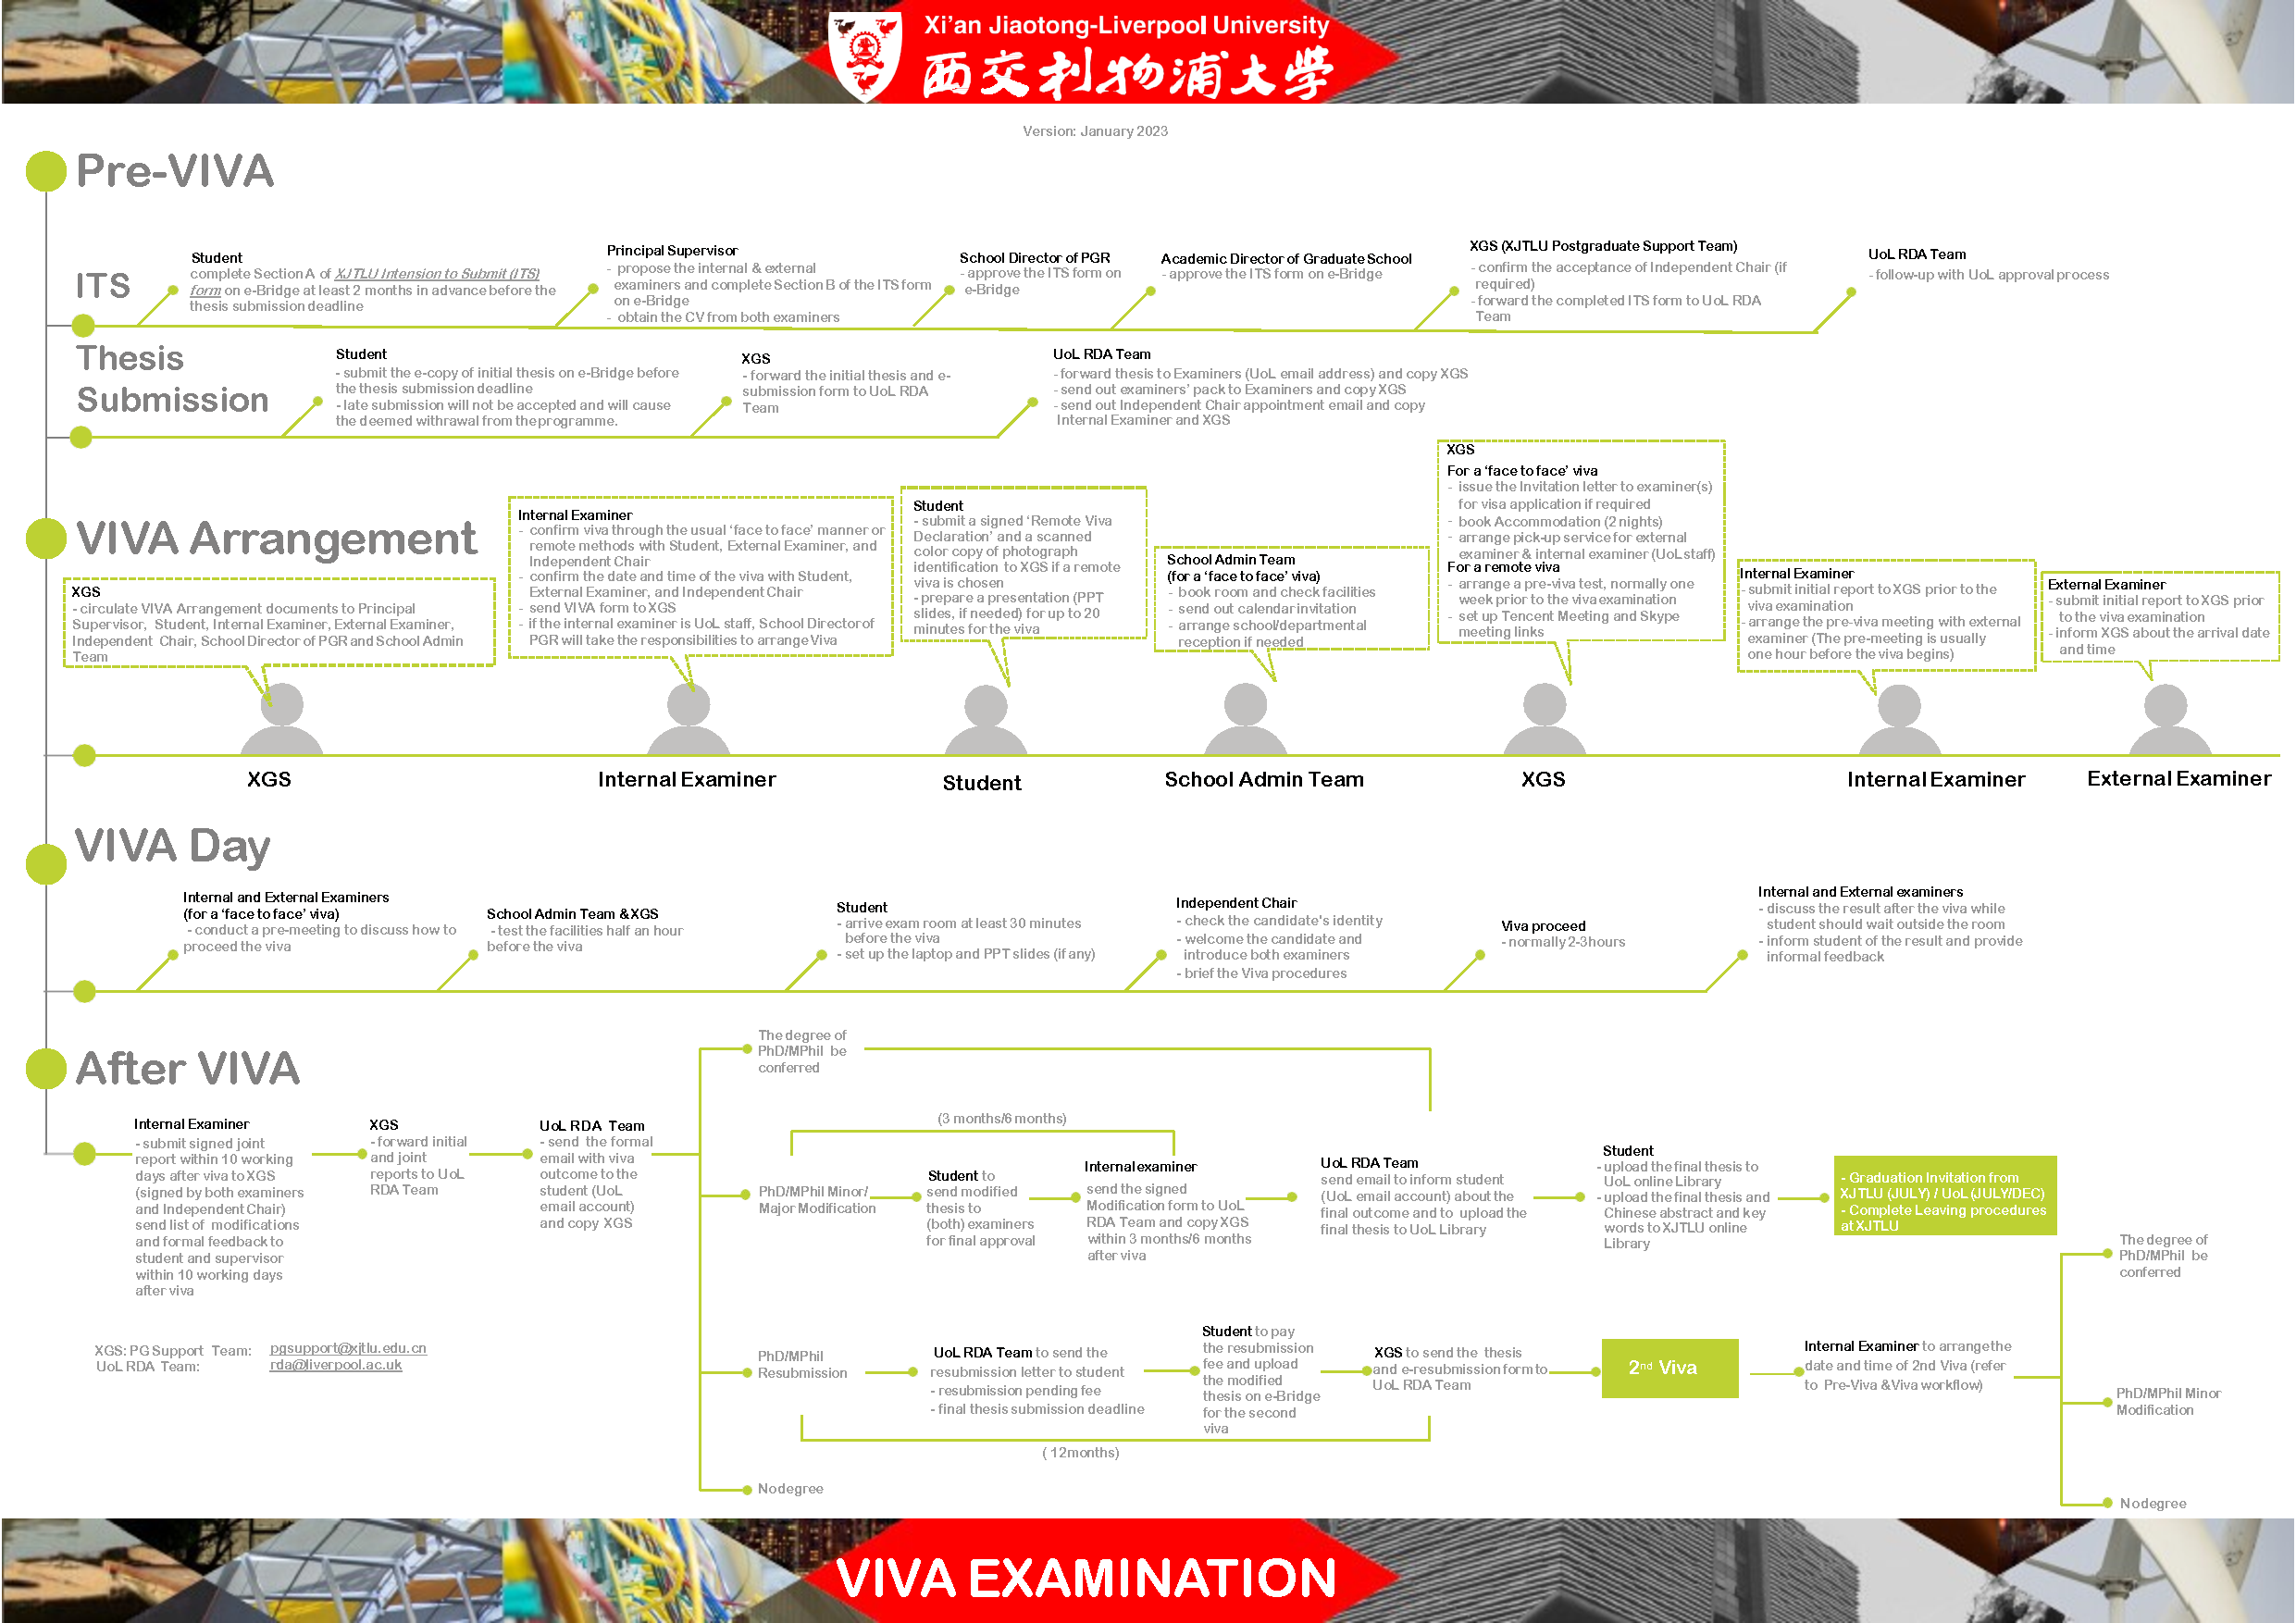
\includegraphics[width=\columnwidth]{fileshare/XJTLU VIVA Examination Arrangement Flowchart_2023.pdf}
    \caption{Official graduation flowchart. The standalone file can be found in the fileshare at \url{https://gitee.com/kaiwu-astro/xp_pgrs_unofficial_guide/tree/main/fileshare}. Note: I don't actually know where this file can be downloaded; this is the one I shared. If you want the latest version, you can look for it on e-bridge.}
\end{figure}

If you want to know approximately how long each step takes, go to Section \ref{sec.graduation.time}.

\subsection{ITS: Intention to Submit}

Q: Is ITS important? I'm eager to write my thesis; can I ignore it for now?

A: If you have requirements regarding your graduation time, please make sure to submit the ITS form as early as possible! ITS is the starting point of all procedures related to your thesis and defense. According to current regulations, you are only allowed to submit your thesis \textbf{at least 2 months after the date of submitting ITS}; you can delay, but you cannot submit earlier. (After submitting ITS, you must submit your thesis within one year; in conjunction with your own thesis deadline, the earlier of the two applies.)

Q: What is included in ITS?

A: The thesis title, thesis abstract, and basic personal information. The title and abstract do not need to be the final versions; they can be modified later.

Q: Then can I just make up a random title and abstract to go through the motions?

A: The purpose of this form is: your supervisor and the Graduate School will use this title and abstract to decide your internal and external examiners. The title and abstract will also be sent to them. Therefore, while modifications are possible compared to the final version, you should still try to accurately reflect your research over the past few years.

Q: I still have questions.

A: First, check the official document: \url{https://www.liverpool.ac.uk/aqsd/academic-codes-of-practice/pgr-code-of-practice/}

\subsection{Thesis: Dissertation/Graduation Thesis}

\subsubsection{Format and Typesetting}

Official document: \url{https://www.liverpool.ac.uk/media/livacuk/tqsd/code-of-practice-on-assessment/annex-7.1-PGR-CoP.pdf}
\newline
For any uncertainties regarding formatting, please refer to this. Below are some frequently asked questions from the group chat.

Q: What software can be used to write the thesis?

A: According to the above regulations, Liverpool has no requirements on software, so you can use whatever you like. Commonly used ones are Microsoft Word and \LaTeX.

Q: What software do you recommend?

A: Advantages of \LaTeX:
\begin{enumerate}
    \item Very convenient for inputting formulas.
    \item References and citations are handled very conveniently, without needing external software like Endnote.
    \item Beautiful formatting, uniform style, and it's hard to make the layout look bad.
    \item Small file size, files can be separated, convenient for backup.
\end{enumerate}
Disadvantages of \LaTeX: High learning curve. If your discipline doesn't use \LaTeX for journal or conference papers and uses Word instead, then you'll need to spend some time learning to switch over.

Q: The formatting requirements in the above document are so many and so detailed. Could you please give me a thesis template?

A:
\begin{enumerate}
    \item There is actually an official Word template, which can be downloaded from the project fileshare at \url{https://gitee.com/kaiwu-astro/xp_pgrs_unofficial_guide/tree/main/fileshare}. Source: Teacher from ELC Thesis Writing Camp.
    \item There is no official \LaTeX\ template, but most graduates from the School of Mathematics and Physics (SMP) use \LaTeX\ to write their theses. You can directly search "Liverpool Thesis" in the Overleaf template library; there should only be one search result.
    \item Students using templates should pay special attention: never fully trust the template! The Word template is provided by ELC teachers at XJTLU, not by Liverpool; the Overleaf one is a community template. In theory, they are \textbf{not responsible} for your thesis and graduation. Therefore, after obtaining a template, the first thing is always to open the Code of Practice above and compare it line by line to see if it meets the requirements.
\end{enumerate}

\subsubsection{Word Count}

Q: The CoP above only mentions an upper word limit; what about the minimum word count?

A: Another frequently asked question. I once asked the teacher in the Graduate School's Thesis Writing Camp course. His opinion was that since XJTLU's Master's thesis has an upper word limit of 30,000, a PhD thesis should preferably exceed this number. But I later found out this is not the case. I have seen theses less than 100 pages, some close to 200 pages, and they all graduated. From the whole university's perspective, there is really no requirement. If you're still worried and want to get an idea of the minimum word count, it's simple: go to the University of Liverpool library and XJTLU library to download theses, focusing on your school, your department, your discipline, preferably theses of your graduated lab mates, and see how many words and pages they have. \textbf{Please remember, having a high word count does not guarantee you can easily graduate}. One of my senior's theses was nearly 200 pages and required major revisions; the external examiner said he wrote too much, like a textbook.

\begin{flushright}
    (August 12, 2024 by \Wu) \\
    (Translated by GPT)
\end{flushright}

\subsection{Thesis Defense}

\subsubsection{Pre- and Post-Defense Process}

\begin{enumerate}
    \item At least two months before officially submitting your thesis on e-bridge, have your supervisor select a list of potential examiners for your upcoming defense. Submit this list to XJTLU's pgsupport and the University of Liverpool for review and approval.
    \item After officially submitting your thesis on e-bridge, the university will contact the respective examiners and then reach out to you to confirm the defense date and format (the defense typically occurs within 1-3 months after submission. The format can be either online or offline — confirm specifics with pgsupport).
    \item Generally, there will be a rehearsal before the defense to test the network and PPT presentation. You can also request time to practice your presentation in the designated conference room.
    \item Before the defense, the examiners will hold an internal meeting, usually on the same day (though sometimes earlier). They will then invite you into the meeting room to officially start the defense. Besides the two (or three under special regulations) examiners, there will be an observer (responsible for overseeing the overall process, arranging breaks, and addressing any procedural questions you might have). During the formal defense, the observer typically does not speak. If you have any questions, feel free to ask them.
    \item After your PPT presentation, there will be a Q\&A session. Depending on the circumstances, this can last from 1.5 to 3.5 hours (historically, there have been instances lasting up to 7 hours). Once the Q\&A concludes, you will be asked to leave the room temporarily while the examiners deliberate. After about 10-15 minutes, you'll be invited back in and informed of the results.
    \item The examiners' revision report will be sent to you within 10 working days. Based on their feedback, you'll need to make the necessary revisions within the specified timeframe and submit them to the primary examiner for confirmation.
    \item Once everything is confirmed, upload the final version of your thesis to complete the process.
\end{enumerate}

\begin{flushright}
    July 5, 2024 by Ziwen Xie \\
    GPT translation proofread by \Shiyao
\end{flushright}

\subsubsection{How to Prepare for a Viva}

Experience from the School of Science:

\textit{Try not to cram everything into a couple of days. Spreading out your preparation helps maintain a good state of mind daily, which is crucial for performing well during the actual defense.}

\textbf{1. Thoroughly read your thesis word by word as if you are a new reader, considering the following questions as you go:}
\begin{enumerate}
    \item Are any paragraphs unclear?
    \item Can you fully grasp and independently explain specific concepts?
    \item Do you understand the relationships and differences between chapters and the internal logic of the overall structure?
    \item Are you aware of the internal logic between sections within chapters and the sequence of experimental designs?
    \item What issues can each experiment address individually or collectively? What conclusions can be drawn from each major chapter?
    \item Do you fully understand the algorithms, models, and basic concepts cited from the literature? How are they connected to your core research objectives?
    \item Are there any previously unnoticed expression errors or chart inaccuracies that need correction?
    \item What is the purpose of your research? What motivated the choice of your methodology? How does it have advantages over other methods?
\end{enumerate}

\textbf{2. After organizing these points, analyze each chapter (including the abstract) in detail:}
\begin{enumerate}
    \item Can you summarize the background information in your own words?
    \item What does each subsection convey? Ensure consistency among subsections within a chapter.
    \item Highlight the key points or core logic of specific experiments or experimental designs.
    \item Understand the progression, parallelism, or other relationships and differences among experimental results (e.g., Experiment A demonstrates 'a', which serves as the foundation for Experiment B—this is progressive. If 'a' and 'b' are similar, then A and B are parallel).
    \item Justify the selection of experimental subjects and models (including why other related subjects or models weren't used).
    \item Based on your results, what future experiments could be pursued? (This may include why certain experiments weren't conducted, reasons for future experiments, potential outcomes of future experiments, foundational assumptions, and practical challenges—which explain why they weren't done in the current phase but were considered).
    \item Ensure the abstract includes key results and innovations.
\end{enumerate}

\textbf{3. Key Points for Preparing Your PPT and Viva:}
\begin{enumerate}
    \item Allocate 20 minutes into four sections: background introduction, experimental setup, experimental results, and conclusions—in approximately 5 minutes each. You can shorten the first three sections since the examiners have already read your thesis.
    \item Print your thesis and bring it with you to the defense. Take notes during the Q\&A session (this also gives you brief moments to compose yourself).
    \item Include essential figures and results in your PPT with concise descriptions.
    \item You don't need to discuss the challenges you faced or focus on future experiments or designs (examiners may ask about these, or you might mention them when answering questions). Depending on the situation, you can omit this from your PPT to save time.
    \item Ensure your PPT runs smoothly, and all text and images are clear. During practice sessions, simulate the actual presentation scenario as closely as possible.
    \item Remember to drink water during the defense—sip slowly and frequently. Eat some high-energy, easily digestible food beforehand. If you're not hungry, consider a chocolate bar or an energizing drink. Arrive early to familiarize yourself with the environment, which can help calm your nerves (and don't forget to visit the restroom beforehand).
    \item When answering questions, feel free to reference any part of your thesis. Some points in earlier chapters may connect with later ones or relate to future plans and final conclusions. If an examiner asks something you're unsure about or haven't considered, it's okay to admit it. Express your willingness to explore it further and ask for guidance or references in their feedback to assist with your revisions.
    \item Typically, each question and answer lasts about 3-5 minutes. With two examiners, handling around 20 questions each is substantial. Usually, the defense lasts between two to two and a half hours, with breaks in between (but once you're engaged, you might lose track of time).
\end{enumerate}

\textbf{4. Non-Thesis Related Questions:}
\begin{enumerate}
    \item How can artificial intelligence and ChatGPT inspire your research?
    \item Can your research be applied to other types of data, diseases, or fields? Why?
    \item What do you think are the shortcomings in your field?
    \item What is your biggest takeaway from your doctoral studies?
    \item If you had to do it all over again, would you still choose to pursue a Ph.D. and undertake this project?
\end{enumerate}
Tips: It seems the examiners are just curious and want a chat. Relax and answer accordingly. \textbf{Finally, according to data from a pgsupport staff member, there has never been a failed defense since our university was established. So, don't worry too much—just perform as you normally would. Good luck.}

\textbf{5. Ask your supervisors if they can help you anticipate potential questions. If time permits, see if they can arrange a mock viva for you (optional). It's also beneficial to consult recent graduates about their defense experiences, as certain aspects may change yearly.}

\begin{flushright}
    July 5, 2024 by Ziwen Xie \\
    GPT translation proofread by \Shiyao
\end{flushright}


\subsection{I Want to Get My Degree Certificate as Soon as Possible! How to Speed Through the Graduation Process}

You're in a hurry—you are the "Hurry King". Below are things a qualified "Hurry King" must know.

\subsubsection{Graduation Certification Documents}

\begin{enumerate}
    \item Completion of Studies Certificate, issued by XJTLU Graduate School. Contents: thesis submitted, defense passed, doctoral degree to be awarded at the graduation ceremony in XXXX year X month. My example:
    \begin{figure}[H]
        \centering
        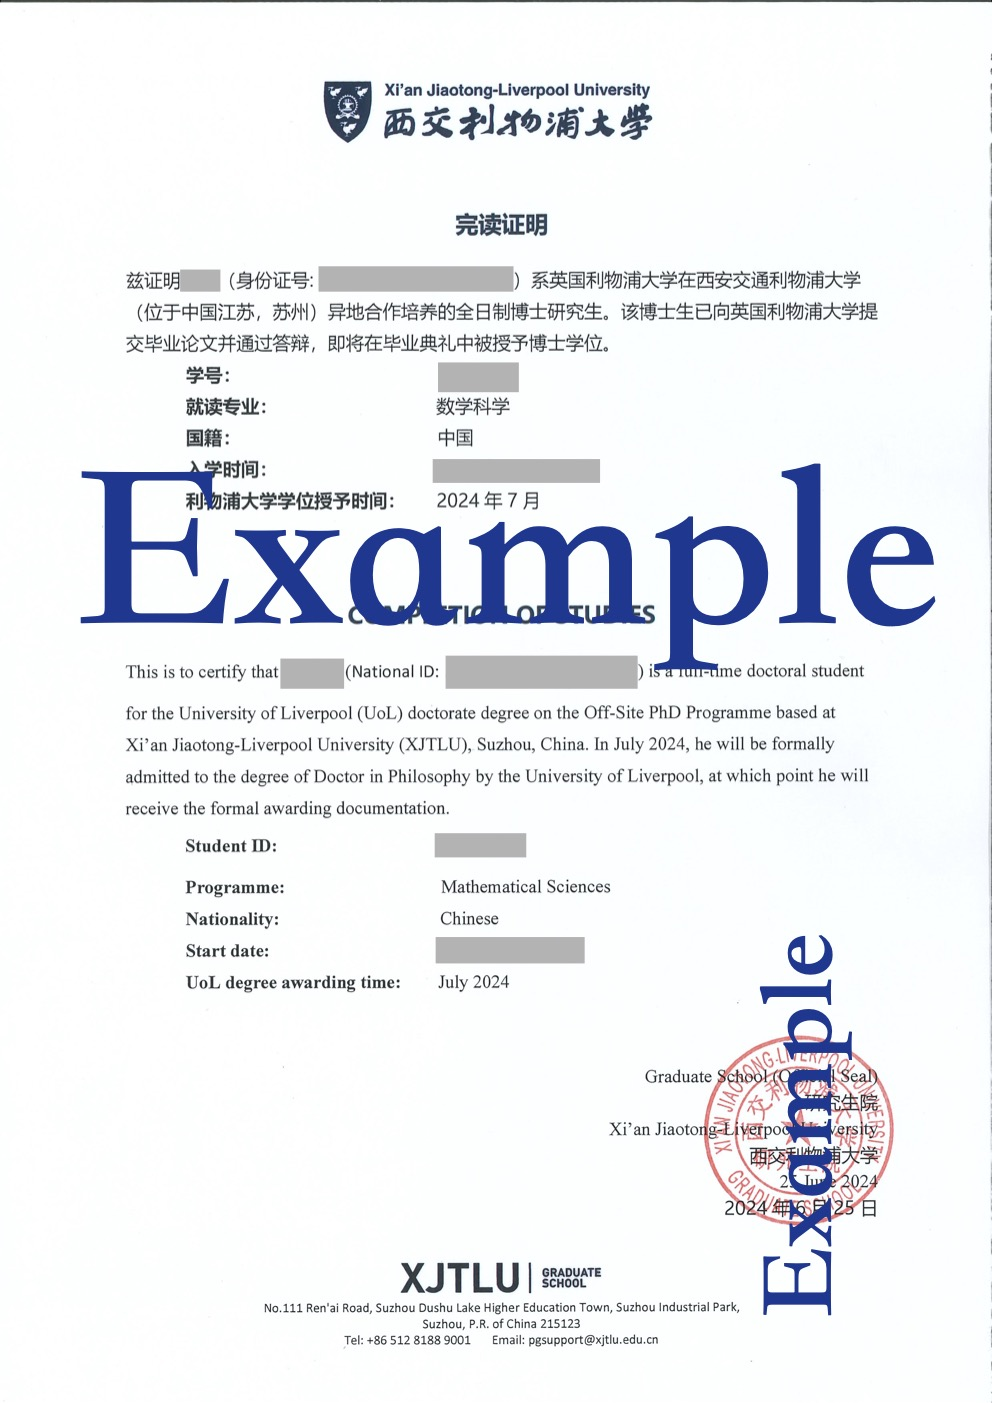
\includegraphics[width=0.8\columnwidth]{author-folder/Kai.Wu/Completion_of_Studies_Certificate_EXAMPLE.jpg}
        \caption{For reference only; a huge "EXAMPLE" is added to prevent illegal use}
    \end{figure}
    \item Degree Certificate (aka PhD degree, degree certificate). Note! According to Liverpool regulations, degrees are only awarded at \textbf{Liverpool} graduation ceremonies, which are held twice a year, usually on certain days in July and December. If you don't attend the Liverpool graduation ceremony, an electronic version of the degree certificate (legally valid and can be used for joint degree authentication) will be issued before and after the graduation ceremony, and then the original will be slowly mailed to XJTLU.
    \item Joint Degree Authentication. With the electronic degree certificate, you can apply at \url{https://zwfw.cscse.edu.cn/}. With this authentication, your Liverpool degree is recognized by the Ministry of Education in China.
\end{enumerate}

Therefore, first determine what certification documents the company or unit you're going to requires. In the most lenient cases, the confirmation email from Liverpool stating you have passed the defense (with minor or major modifications) after the defense is sufficient. Some may accept the Completion of Studies Certificate. If the other party is more stringent and won't accept anything less than the degree certificate, or even the joint degree authentication, then you need to plan your graduation progress carefully because degrees are only awarded twice a year!

\subsubsection{Degree Certificate: The Most Critical Time Nodes}

If you're sure you don't need to rush to get the degree certificate, you can ignore the rest of this section because the Completion of Studies Certificate can be issued at any time.

Q: Can I graduate in July or December? What are the hard requirements?

A: The best way is to check directly on the Liverpool website or just Google "Liverpool PhD graduation". In recent years, the requirement has been: before a certain date, the University of Liverpool library must confirm receipt of your \sout{final, completely unmodifiable} final thesis. For example, to participate in the July 15, 2024, Liverpool graduation ceremony (degree certificate awarded or mailed on that day), the Liverpool library must confirm receipt of your final thesis by June 25, 2024. This thesis is the final version agreed upon by both your internal and external examiners. How do you reach this point? See the next section.

\subsubsection{How Long Does Each Step Take? How to Estimate the Time?}
\label{sec.graduation.time}

The following is entirely based on the experiences of already graduated students. New graduates, please feel free to contribute and supplement your real cases.

Let's go through the flowchart mentioned in Section \ref{sec.official.flowchart}:

\begin{enumerate}
    \item ITS: After you submit, you don't need to worry about it anymore; focus on writing your thesis—the rest is your supervisor's and the Graduate School's work. Behind the scenes:
    \begin{enumerate}
        \item Supervisor proposes internal and external examiners.
        \item Graduate School reviews and may reject any of them if it considers the examiner has a conflict of interest; then your supervisor re-proposes until the Graduate School is satisfied, finalizing one internal and one external examiner.
    \end{enumerate}
    At this stage, strictly speaking, you won't know who your internal and external examiners are until you submit your thesis; your supervisor needs to keep it confidential, so don't \textbf{overly} press your supervisor to tell you who they are.
    \item From first thesis submission to thesis defense (30 days ± 30 days): After submission, XJTLU Graduate School (XGS) and Liverpool's Research Degree Administration (RDA) will take two or three working days to process your thesis and send it to the internal and external examiners. \textbf{The internal examiner}, once they receive the thesis, is responsible for arranging the defense date. In other words, your defense date depends entirely on when you, the internal examiner, the external examiner, and the independent chair all have time (normally 2–3 hours). Therefore, the earliest defense date is three or four working days after submission; there is no specified latest defense date—until all four people have time. If you're in a hurry, what you can do:
    \begin{enumerate}
        \item After thesis submission, contact your internal examiner as soon as possible to urge them to arrange a date.
        \item Try to free up your schedule in the one or two months after thesis submission so that your availability doesn't delay the defense.
        \item Once the internal and external examiners are set, it's hard to change them, but the independent chair is easier to replace (sometimes a week before the defense, the chair may not be available and another teacher steps in). If among the four of you, it's the chair's schedule causing delays, consider asking your supervisor if the chair can be changed.
    \end{enumerate}
    Normally, submitting the thesis plus 60 days until defense is considered very slow (but there are examples; it's said that the defense was delayed as it coincided with strikes at Liverpool around the submission time). Generally, it's around 30 days.
    \item From defense completion to final thesis approval (0–180 days, typically 3–4 weeks): This step varies greatly depending on the defense outcome.
    \begin{enumerate}
        \item Pass (unconditional): 0 days; the initial version of the thesis is the final version.
        \item Pass with minor modifications: the result for the vast majority of students.
        \item Pass with major modifications (other more unfortunate cases are rare, \sout{suggest your supervisor fight with the examiner they recommended}).
    \end{enumerate}
    If it's (2) or (3), the internal and external examiners will provide a written modification report within 10 working days (2 weeks). My personal suggestion is not to rush this process; they have quite a few forms and reports to submit. After that, how quickly you revise the thesis depends on you. After revising, send the revised thesis to the examiners as per Liverpool's email instructions. This step entirely depends on how long it takes your internal and external examiners to respond and whether they are satisfied with your revisions. According to the process, if they are not satisfied, they have the right to ask you to revise until they are satisfied. To avoid iterative back-and-forth, it's suggested to carefully consider the new text with your supervisor to strive to get it right in one go. This version of the thesis will not automatically be the final version; you can use colors or bold to highlight the modified parts, making it easier for the two examiners to review.
    \item From final thesis approval to Liverpool library confirmation of receipt (7 days): This step is just administrative procedure. After approval, RDA will send you an email to inform you to upload the final thesis (in my case, the internal examiner told me [they have notified XGS and RDA that the revised version is approved], and after 4 days, I received the upload notice). Then you send the final thesis to Liverpool, and after a few days (in my case, 2 days), you receive formal notification from the Liverpool library that the thesis has been successfully uploaded.
    \item There are actually some other procedures, such as XJTLU also asking you to upload a copy to their library. I don't know if it affects graduation, but it's best to complete it as soon as you receive the notification.
    \item Electronic degree: The legally valid electronic degree certificate will be issued a few days before or after your graduation ceremony date. According to the email from Liverpool, check at \url{verify.liverpool.ac.uk}.
    \item Paper degree: If you attend the graduation ceremony at Liverpool in person, you can collect it on-site. If you don't go, it will be officially mailed to XJTLU after your graduation ceremony date. Just wait for it. In my case: July 15 was the Liverpool graduation ceremony (I didn't go), and the paper version arrived at the Graduate School on July 30. If you are no longer at the university by then, you can entrust the Graduate School to mail it (not recommended, as loss of the document cannot be compensated, and the risk is on you).
\end{enumerate}

\begin{flushright}
    (August 12, 2024 by \Wu) \\
    (Translated by GPT)
\end{flushright}